\documentclass[twoside]{book}

% Packages required by doxygen
\usepackage{fixltx2e}
\usepackage{calc}
\usepackage{doxygen}
\usepackage[export]{adjustbox} % also loads graphicx
\usepackage{graphicx}
\usepackage[utf8]{inputenc}
\usepackage{makeidx}
\usepackage{multicol}
\usepackage{multirow}
\PassOptionsToPackage{warn}{textcomp}
\usepackage{textcomp}
\usepackage[nointegrals]{wasysym}
\usepackage[table]{xcolor}

% NLS support packages
\usepackage[ngerman]{babel}

% Font selection
\usepackage[T1]{fontenc}
\usepackage[scaled=.90]{helvet}
\usepackage{courier}
\usepackage{amssymb}
\usepackage{sectsty}
\renewcommand{\familydefault}{\sfdefault}
\allsectionsfont{%
  \fontseries{bc}\selectfont%
  \color{darkgray}%
}
\renewcommand{\DoxyLabelFont}{%
  \fontseries{bc}\selectfont%
  \color{darkgray}%
}
\newcommand{\+}{\discretionary{\mbox{\scriptsize$\hookleftarrow$}}{}{}}

% Page & text layout
\usepackage{geometry}
\geometry{%
  a4paper,%
  top=2.5cm,%
  bottom=2.5cm,%
  left=2.5cm,%
  right=2.5cm%
}
\tolerance=750
\hfuzz=15pt
\hbadness=750
\setlength{\emergencystretch}{15pt}
\setlength{\parindent}{0cm}
\setlength{\parskip}{3ex plus 2ex minus 2ex}
\makeatletter
\renewcommand{\paragraph}{%
  \@startsection{paragraph}{4}{0ex}{-1.0ex}{1.0ex}{%
    \normalfont\normalsize\bfseries\SS@parafont%
  }%
}
\renewcommand{\subparagraph}{%
  \@startsection{subparagraph}{5}{0ex}{-1.0ex}{1.0ex}{%
    \normalfont\normalsize\bfseries\SS@subparafont%
  }%
}
\makeatother

% Headers & footers
\usepackage{fancyhdr}
\pagestyle{fancyplain}
\fancyhead[LE]{\fancyplain{}{\bfseries\thepage}}
\fancyhead[CE]{\fancyplain{}{}}
\fancyhead[RE]{\fancyplain{}{\bfseries\leftmark}}
\fancyhead[LO]{\fancyplain{}{\bfseries\rightmark}}
\fancyhead[CO]{\fancyplain{}{}}
\fancyhead[RO]{\fancyplain{}{\bfseries\thepage}}
\fancyfoot[LE]{\fancyplain{}{}}
\fancyfoot[CE]{\fancyplain{}{}}
\fancyfoot[RE]{\fancyplain{}{\bfseries\scriptsize Erzeugt von Doxygen }}
\fancyfoot[LO]{\fancyplain{}{\bfseries\scriptsize Erzeugt von Doxygen }}
\fancyfoot[CO]{\fancyplain{}{}}
\fancyfoot[RO]{\fancyplain{}{}}
\renewcommand{\footrulewidth}{0.4pt}
\renewcommand{\chaptermark}[1]{%
  \markboth{#1}{}%
}
\renewcommand{\sectionmark}[1]{%
  \markright{\thesection\ #1}%
}

% Indices & bibliography
\usepackage{natbib}
\usepackage[titles]{tocloft}
\setcounter{tocdepth}{3}
\setcounter{secnumdepth}{5}
\makeindex

% Hyperlinks (required, but should be loaded last)
\usepackage{ifpdf}
\ifpdf
  \usepackage[pdftex,pagebackref=true]{hyperref}
\else
  \usepackage[ps2pdf,pagebackref=true]{hyperref}
\fi
\hypersetup{%
  colorlinks=true,%
  linkcolor=blue,%
  citecolor=blue,%
  unicode%
}

% Custom commands
\newcommand{\clearemptydoublepage}{%
  \newpage{\pagestyle{empty}\cleardoublepage}%
}

\usepackage{caption}
\captionsetup{labelsep=space,justification=centering,font={bf},singlelinecheck=off,skip=4pt,position=top}

%===== C O N T E N T S =====

\begin{document}

% Titlepage & ToC
\hypersetup{pageanchor=false,
             bookmarksnumbered=true,
             pdfencoding=unicode
            }
\pagenumbering{alph}
\begin{titlepage}
\vspace*{7cm}
\begin{center}%
{\Large Robot Arm \\[1ex]\large 1.\+0.\+0 }\\
\vspace*{1cm}
{\large Erzeugt von Doxygen 1.8.13}\\
\end{center}
\end{titlepage}
\clearemptydoublepage
\pagenumbering{roman}
\tableofcontents
\clearemptydoublepage
\pagenumbering{arabic}
\hypersetup{pageanchor=true}

%--- Begin generated contents ---
\chapter{Verzeichnis der Namensbereiche}
\section{Pakete}
Hier folgen die Pakete mit einer Kurzbeschreibung (wenn verfügbar)\+:\begin{DoxyCompactList}
\item\contentsline{section}{\hyperlink{namespace_f_i_n_a_l___g_u_i___w_l_a_n}{F\+I\+N\+A\+L\+\_\+\+G\+U\+I\+\_\+\+W\+L\+AN} }{\pageref{namespace_f_i_n_a_l___g_u_i___w_l_a_n}}{}
\end{DoxyCompactList}

\chapter{Hierarchie-\/\+Verzeichnis}
\section{Class Hierarchy}
This inheritance list is sorted roughly, but not completely, alphabetically\+:\begin{DoxyCompactList}
\item object\begin{DoxyCompactList}
\item \contentsline{section}{F\+I\+N\+A\+L\+\_\+\+G\+U\+I\+\_\+\+W\+L\+A\+N.\+Arduino}{\pageref{class_f_i_n_a_l___g_u_i___w_l_a_n_1_1_arduino}}{}
\item \contentsline{section}{F\+I\+N\+A\+L\+\_\+\+G\+U\+I\+\_\+\+W\+L\+A\+N.\+W\+L\+AN}{\pageref{class_f_i_n_a_l___g_u_i___w_l_a_n_1_1_w_l_a_n}}{}
\end{DoxyCompactList}
\end{DoxyCompactList}

\chapter{Klassen-\/\+Verzeichnis}
\section{Class List}
Here are the classes, structs, unions and interfaces with brief descriptions\+:\begin{DoxyCompactList}
\item\contentsline{section}{\hyperlink{class_f_i_n_a_l___g_u_i___w_l_a_n_1_1_arduino}{F\+I\+N\+A\+L\+\_\+\+G\+U\+I\+\_\+\+W\+L\+A\+N.\+Arduino} }{\pageref{class_f_i_n_a_l___g_u_i___w_l_a_n_1_1_arduino}}{}
\item\contentsline{section}{\hyperlink{class_f_i_n_a_l___g_u_i___w_l_a_n_1_1_w_l_a_n}{F\+I\+N\+A\+L\+\_\+\+G\+U\+I\+\_\+\+W\+L\+A\+N.\+W\+L\+AN} }{\pageref{class_f_i_n_a_l___g_u_i___w_l_a_n_1_1_w_l_a_n}}{}
\end{DoxyCompactList}

\chapter{Datei-\/\+Verzeichnis}
\section{Auflistung der Dateien}
Hier folgt die Aufzählung aller Dateien mit einer Kurzbeschreibung\+:\begin{DoxyCompactList}
\item\contentsline{section}{Arduino\+\_\+kommentiert/\hyperlink{_arduino__kommentiert_8ino}{Arduino\+\_\+kommentiert.\+ino} }{\pageref{_arduino__kommentiert_8ino}}{}
\item\contentsline{section}{Arduino\+\_\+kommentiert/\hyperlink{_dumb_server_8cpp}{Dumb\+Server.\+cpp} }{\pageref{_dumb_server_8cpp}}{}
\item\contentsline{section}{Arduino\+\_\+kommentiert/\hyperlink{_dumb_server_8h}{Dumb\+Server.\+h} }{\pageref{_dumb_server_8h}}{}
\end{DoxyCompactList}

\chapter{Dokumentation der Namensbereiche}
\hypertarget{namespace_f_i_n_a_l___g_u_i___w_l_a_n}{}\section{F\+I\+N\+A\+L\+\_\+\+G\+U\+I\+\_\+\+W\+L\+A\+N-\/\+Namensbereichsreferenz}
\label{namespace_f_i_n_a_l___g_u_i___w_l_a_n}\index{F\+I\+N\+A\+L\+\_\+\+G\+U\+I\+\_\+\+W\+L\+AN@{F\+I\+N\+A\+L\+\_\+\+G\+U\+I\+\_\+\+W\+L\+AN}}
\subsection*{Datenstrukturen}
\begin{DoxyCompactItemize}
\item 
class \hyperlink{class_f_i_n_a_l___g_u_i___w_l_a_n_1_1_arduino}{Arduino}
\item 
class \hyperlink{class_f_i_n_a_l___g_u_i___w_l_a_n_1_1_w_l_a_n}{W\+L\+AN}
\end{DoxyCompactItemize}
\subsection*{Variablen}
\begin{DoxyCompactItemize}
\item 
\hyperlink{namespace_f_i_n_a_l___g_u_i___w_l_a_n_a04a8a2bbfa9c15500892b8e5033d625b}{window} = \hyperlink{class_f_i_n_a_l___g_u_i___w_l_a_n_1_1_w_l_a_n}{W\+L\+AN}()
\end{DoxyCompactItemize}


\subsection{Variablen-\/\+Dokumentation}
\mbox{\Hypertarget{namespace_f_i_n_a_l___g_u_i___w_l_a_n_a04a8a2bbfa9c15500892b8e5033d625b}\label{namespace_f_i_n_a_l___g_u_i___w_l_a_n_a04a8a2bbfa9c15500892b8e5033d625b}} 
\index{F\+I\+N\+A\+L\+\_\+\+G\+U\+I\+\_\+\+W\+L\+AN@{F\+I\+N\+A\+L\+\_\+\+G\+U\+I\+\_\+\+W\+L\+AN}!window@{window}}
\index{window@{window}!F\+I\+N\+A\+L\+\_\+\+G\+U\+I\+\_\+\+W\+L\+AN@{F\+I\+N\+A\+L\+\_\+\+G\+U\+I\+\_\+\+W\+L\+AN}}
\subsubsection{\texorpdfstring{window}{window}}
{\footnotesize\ttfamily window = \hyperlink{class_f_i_n_a_l___g_u_i___w_l_a_n_1_1_w_l_a_n}{W\+L\+AN}()}



Definiert in Zeile 249 der Datei F\+I\+N\+A\+L\+\_\+\+G\+U\+I\+\_\+\+W\+L\+A\+N.\+py.


\chapter{Klassen-\/\+Dokumentation}
\hypertarget{class_f_i_n_a_l___g_u_i___w_l_a_n_1_1_arduino}{}\section{F\+I\+N\+A\+L\+\_\+\+G\+U\+I\+\_\+\+W\+L\+A\+N.\+Arduino Klassenreferenz}
\label{class_f_i_n_a_l___g_u_i___w_l_a_n_1_1_arduino}\index{F\+I\+N\+A\+L\+\_\+\+G\+U\+I\+\_\+\+W\+L\+A\+N.\+Arduino@{F\+I\+N\+A\+L\+\_\+\+G\+U\+I\+\_\+\+W\+L\+A\+N.\+Arduino}}


Klassendiagramm für F\+I\+N\+A\+L\+\_\+\+G\+U\+I\+\_\+\+W\+L\+A\+N.\+Arduino\+:\nopagebreak
\begin{figure}[H]
\begin{center}
\leavevmode
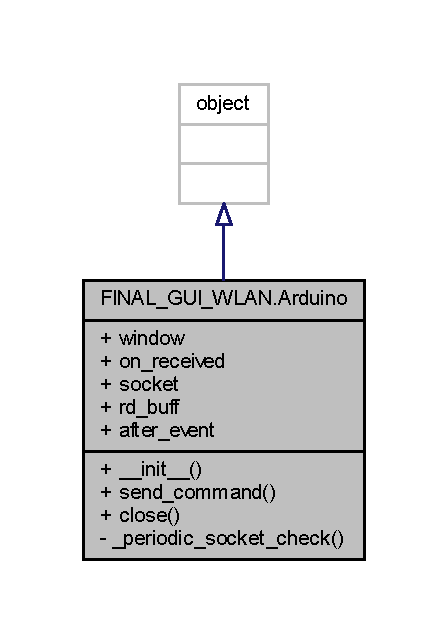
\includegraphics[width=215pt]{class_f_i_n_a_l___g_u_i___w_l_a_n_1_1_arduino__inherit__graph}
\end{center}
\end{figure}


Zusammengehörigkeiten von F\+I\+N\+A\+L\+\_\+\+G\+U\+I\+\_\+\+W\+L\+A\+N.\+Arduino\+:\nopagebreak
\begin{figure}[H]
\begin{center}
\leavevmode
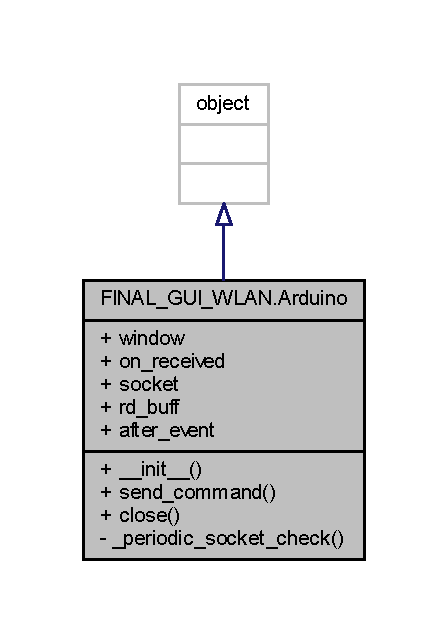
\includegraphics[width=215pt]{class_f_i_n_a_l___g_u_i___w_l_a_n_1_1_arduino__coll__graph}
\end{center}
\end{figure}
\subsection*{Öffentliche Methoden}
\begin{DoxyCompactItemize}
\item 
def \hyperlink{class_f_i_n_a_l___g_u_i___w_l_a_n_1_1_arduino_ac826ff80647459671ac4367c0c11b7b1}{\+\_\+\+\_\+init\+\_\+\+\_\+} (self, \hyperlink{class_f_i_n_a_l___g_u_i___w_l_a_n_1_1_arduino_a731b3fc58c501b945f1df4d2e8120112}{window}, host, port, \hyperlink{class_f_i_n_a_l___g_u_i___w_l_a_n_1_1_arduino_aecdaccc57653078abe4ffe967cba361e}{on\+\_\+received})
\item 
def \hyperlink{class_f_i_n_a_l___g_u_i___w_l_a_n_1_1_arduino_a2a13c6006cd466ac37ce8e2033d04e96}{send\+\_\+command} (self, command)
\item 
def \hyperlink{class_f_i_n_a_l___g_u_i___w_l_a_n_1_1_arduino_a07b83bfe05b0faf47ad2e6730d3ae795}{close} (self)
\end{DoxyCompactItemize}
\subsection*{Öffentliche Attribute}
\begin{DoxyCompactItemize}
\item 
\hyperlink{class_f_i_n_a_l___g_u_i___w_l_a_n_1_1_arduino_a731b3fc58c501b945f1df4d2e8120112}{window}
\item 
\hyperlink{class_f_i_n_a_l___g_u_i___w_l_a_n_1_1_arduino_aecdaccc57653078abe4ffe967cba361e}{on\+\_\+received}
\item 
\hyperlink{class_f_i_n_a_l___g_u_i___w_l_a_n_1_1_arduino_a0728cfa43c874b9a4b8389f4b3215df0}{socket}
\item 
\hyperlink{class_f_i_n_a_l___g_u_i___w_l_a_n_1_1_arduino_a220d4f39773ac5352c7ce4cd4bb89b7d}{rd\+\_\+buff}
\item 
\hyperlink{class_f_i_n_a_l___g_u_i___w_l_a_n_1_1_arduino_a7858221e882d55f393ce792d56115341}{after\+\_\+event}
\end{DoxyCompactItemize}
\subsection*{Private Methoden}
\begin{DoxyCompactItemize}
\item 
def \hyperlink{class_f_i_n_a_l___g_u_i___w_l_a_n_1_1_arduino_a870ded4eb313dea386ae38c6c6267bbf}{\+\_\+periodic\+\_\+socket\+\_\+check} (self)
\end{DoxyCompactItemize}


\subsection{Ausführliche Beschreibung}


Definiert in Zeile 7 der Datei F\+I\+N\+A\+L\+\_\+\+G\+U\+I\+\_\+\+W\+L\+A\+N.\+py.



\subsection{Beschreibung der Konstruktoren und Destruktoren}
\mbox{\Hypertarget{class_f_i_n_a_l___g_u_i___w_l_a_n_1_1_arduino_ac826ff80647459671ac4367c0c11b7b1}\label{class_f_i_n_a_l___g_u_i___w_l_a_n_1_1_arduino_ac826ff80647459671ac4367c0c11b7b1}} 
\index{F\+I\+N\+A\+L\+\_\+\+G\+U\+I\+\_\+\+W\+L\+A\+N\+::\+Arduino@{F\+I\+N\+A\+L\+\_\+\+G\+U\+I\+\_\+\+W\+L\+A\+N\+::\+Arduino}!\+\_\+\+\_\+init\+\_\+\+\_\+@{\+\_\+\+\_\+init\+\_\+\+\_\+}}
\index{\+\_\+\+\_\+init\+\_\+\+\_\+@{\+\_\+\+\_\+init\+\_\+\+\_\+}!F\+I\+N\+A\+L\+\_\+\+G\+U\+I\+\_\+\+W\+L\+A\+N\+::\+Arduino@{F\+I\+N\+A\+L\+\_\+\+G\+U\+I\+\_\+\+W\+L\+A\+N\+::\+Arduino}}
\subsubsection{\texorpdfstring{\+\_\+\+\_\+init\+\_\+\+\_\+()}{\_\_init\_\_()}}
{\footnotesize\ttfamily def F\+I\+N\+A\+L\+\_\+\+G\+U\+I\+\_\+\+W\+L\+A\+N.\+Arduino.\+\_\+\+\_\+init\+\_\+\+\_\+ (\begin{DoxyParamCaption}\item[{}]{self,  }\item[{}]{window,  }\item[{}]{host,  }\item[{}]{port,  }\item[{}]{on\+\_\+received }\end{DoxyParamCaption})}



Definiert in Zeile 8 der Datei F\+I\+N\+A\+L\+\_\+\+G\+U\+I\+\_\+\+W\+L\+A\+N.\+py.


\begin{DoxyCode}
8     \textcolor{keyword}{def }\_\_init\_\_(self, window, host, port, on\_received):
9         self.window= window
10         self.on\_received= on\_received
11 
12         self.socket= so.socket()
13         self.socket.connect((\textcolor{stringliteral}{'170.20.10.5'}, 30304))    \textcolor{stringliteral}{"""Für die Verbindung mit dem WLAN Shield"""}
14         self.socket.setblocking(\textcolor{keyword}{False})
15 
16         self.rd\_buff= bytes()
17 
18         self.\_periodic\_socket\_check()
19 
\end{DoxyCode}


\subsection{Dokumentation der Elementfunktionen}
\mbox{\Hypertarget{class_f_i_n_a_l___g_u_i___w_l_a_n_1_1_arduino_a870ded4eb313dea386ae38c6c6267bbf}\label{class_f_i_n_a_l___g_u_i___w_l_a_n_1_1_arduino_a870ded4eb313dea386ae38c6c6267bbf}} 
\index{F\+I\+N\+A\+L\+\_\+\+G\+U\+I\+\_\+\+W\+L\+A\+N\+::\+Arduino@{F\+I\+N\+A\+L\+\_\+\+G\+U\+I\+\_\+\+W\+L\+A\+N\+::\+Arduino}!\+\_\+periodic\+\_\+socket\+\_\+check@{\+\_\+periodic\+\_\+socket\+\_\+check}}
\index{\+\_\+periodic\+\_\+socket\+\_\+check@{\+\_\+periodic\+\_\+socket\+\_\+check}!F\+I\+N\+A\+L\+\_\+\+G\+U\+I\+\_\+\+W\+L\+A\+N\+::\+Arduino@{F\+I\+N\+A\+L\+\_\+\+G\+U\+I\+\_\+\+W\+L\+A\+N\+::\+Arduino}}
\subsubsection{\texorpdfstring{\+\_\+periodic\+\_\+socket\+\_\+check()}{\_periodic\_socket\_check()}}
{\footnotesize\ttfamily def F\+I\+N\+A\+L\+\_\+\+G\+U\+I\+\_\+\+W\+L\+A\+N.\+Arduino.\+\_\+periodic\+\_\+socket\+\_\+check (\begin{DoxyParamCaption}\item[{}]{self }\end{DoxyParamCaption})\hspace{0.3cm}{\ttfamily [private]}}



Definiert in Zeile 30 der Datei F\+I\+N\+A\+L\+\_\+\+G\+U\+I\+\_\+\+W\+L\+A\+N.\+py.


\begin{DoxyCode}
30     \textcolor{keyword}{def }\_periodic\_socket\_check(self):
31         \textcolor{keywordflow}{try}:
32             msg= self.socket.recv(1024)
33 
34             \textcolor{keywordflow}{if} \textcolor{keywordflow}{not} msg:
35                 raise(IOError(\textcolor{stringliteral}{'Connection closed'}))
36 
37             self.rd\_buff+= msg
38 
39         \textcolor{keywordflow}{except} so.error:
40             \textcolor{keywordflow}{pass}
41 
42         \textcolor{keywordflow}{while} b\textcolor{stringliteral}{'\(\backslash\)n'} \textcolor{keywordflow}{in} self.rd\_buff:
43             line, self.rd\_buff= self.rd\_buff.split(b\textcolor{stringliteral}{'\(\backslash\)n'})
44 
45             line= line.decode(\textcolor{stringliteral}{'utf-8'}).strip()
46             self.on\_received(line)
47 
48         self.after\_event= self.window.after(
49             100, self.\_periodic\_socket\_check
50         )
51 
52 
53 
\end{DoxyCode}
\mbox{\Hypertarget{class_f_i_n_a_l___g_u_i___w_l_a_n_1_1_arduino_a07b83bfe05b0faf47ad2e6730d3ae795}\label{class_f_i_n_a_l___g_u_i___w_l_a_n_1_1_arduino_a07b83bfe05b0faf47ad2e6730d3ae795}} 
\index{F\+I\+N\+A\+L\+\_\+\+G\+U\+I\+\_\+\+W\+L\+A\+N\+::\+Arduino@{F\+I\+N\+A\+L\+\_\+\+G\+U\+I\+\_\+\+W\+L\+A\+N\+::\+Arduino}!close@{close}}
\index{close@{close}!F\+I\+N\+A\+L\+\_\+\+G\+U\+I\+\_\+\+W\+L\+A\+N\+::\+Arduino@{F\+I\+N\+A\+L\+\_\+\+G\+U\+I\+\_\+\+W\+L\+A\+N\+::\+Arduino}}
\subsubsection{\texorpdfstring{close()}{close()}}
{\footnotesize\ttfamily def F\+I\+N\+A\+L\+\_\+\+G\+U\+I\+\_\+\+W\+L\+A\+N.\+Arduino.\+close (\begin{DoxyParamCaption}\item[{}]{self }\end{DoxyParamCaption})}



Definiert in Zeile 25 der Datei F\+I\+N\+A\+L\+\_\+\+G\+U\+I\+\_\+\+W\+L\+A\+N.\+py.


\begin{DoxyCode}
25     \textcolor{keyword}{def }close(self):
26 
27         self.socket.close()                            \textcolor{stringliteral}{"""Damit die GUI geschlossen werden kann"""}
28         self.window.after\_cancel(self.after\_event)
29 
\end{DoxyCode}
\mbox{\Hypertarget{class_f_i_n_a_l___g_u_i___w_l_a_n_1_1_arduino_a2a13c6006cd466ac37ce8e2033d04e96}\label{class_f_i_n_a_l___g_u_i___w_l_a_n_1_1_arduino_a2a13c6006cd466ac37ce8e2033d04e96}} 
\index{F\+I\+N\+A\+L\+\_\+\+G\+U\+I\+\_\+\+W\+L\+A\+N\+::\+Arduino@{F\+I\+N\+A\+L\+\_\+\+G\+U\+I\+\_\+\+W\+L\+A\+N\+::\+Arduino}!send\+\_\+command@{send\+\_\+command}}
\index{send\+\_\+command@{send\+\_\+command}!F\+I\+N\+A\+L\+\_\+\+G\+U\+I\+\_\+\+W\+L\+A\+N\+::\+Arduino@{F\+I\+N\+A\+L\+\_\+\+G\+U\+I\+\_\+\+W\+L\+A\+N\+::\+Arduino}}
\subsubsection{\texorpdfstring{send\+\_\+command()}{send\_command()}}
{\footnotesize\ttfamily def F\+I\+N\+A\+L\+\_\+\+G\+U\+I\+\_\+\+W\+L\+A\+N.\+Arduino.\+send\+\_\+command (\begin{DoxyParamCaption}\item[{}]{self,  }\item[{}]{command }\end{DoxyParamCaption})}



Definiert in Zeile 20 der Datei F\+I\+N\+A\+L\+\_\+\+G\+U\+I\+\_\+\+W\+L\+A\+N.\+py.


\begin{DoxyCode}
20     \textcolor{keyword}{def }send\_command(self, command):
21 
22 
23         self.socket.send(command.encode(\textcolor{stringliteral}{'utf-8'}) + b\textcolor{stringliteral}{'\(\backslash\)n'})
24 
\end{DoxyCode}


\subsection{Dokumentation der Datenelemente}
\mbox{\Hypertarget{class_f_i_n_a_l___g_u_i___w_l_a_n_1_1_arduino_a7858221e882d55f393ce792d56115341}\label{class_f_i_n_a_l___g_u_i___w_l_a_n_1_1_arduino_a7858221e882d55f393ce792d56115341}} 
\index{F\+I\+N\+A\+L\+\_\+\+G\+U\+I\+\_\+\+W\+L\+A\+N\+::\+Arduino@{F\+I\+N\+A\+L\+\_\+\+G\+U\+I\+\_\+\+W\+L\+A\+N\+::\+Arduino}!after\+\_\+event@{after\+\_\+event}}
\index{after\+\_\+event@{after\+\_\+event}!F\+I\+N\+A\+L\+\_\+\+G\+U\+I\+\_\+\+W\+L\+A\+N\+::\+Arduino@{F\+I\+N\+A\+L\+\_\+\+G\+U\+I\+\_\+\+W\+L\+A\+N\+::\+Arduino}}
\subsubsection{\texorpdfstring{after\+\_\+event}{after\_event}}
{\footnotesize\ttfamily F\+I\+N\+A\+L\+\_\+\+G\+U\+I\+\_\+\+W\+L\+A\+N.\+Arduino.\+after\+\_\+event}



Definiert in Zeile 48 der Datei F\+I\+N\+A\+L\+\_\+\+G\+U\+I\+\_\+\+W\+L\+A\+N.\+py.

\mbox{\Hypertarget{class_f_i_n_a_l___g_u_i___w_l_a_n_1_1_arduino_aecdaccc57653078abe4ffe967cba361e}\label{class_f_i_n_a_l___g_u_i___w_l_a_n_1_1_arduino_aecdaccc57653078abe4ffe967cba361e}} 
\index{F\+I\+N\+A\+L\+\_\+\+G\+U\+I\+\_\+\+W\+L\+A\+N\+::\+Arduino@{F\+I\+N\+A\+L\+\_\+\+G\+U\+I\+\_\+\+W\+L\+A\+N\+::\+Arduino}!on\+\_\+received@{on\+\_\+received}}
\index{on\+\_\+received@{on\+\_\+received}!F\+I\+N\+A\+L\+\_\+\+G\+U\+I\+\_\+\+W\+L\+A\+N\+::\+Arduino@{F\+I\+N\+A\+L\+\_\+\+G\+U\+I\+\_\+\+W\+L\+A\+N\+::\+Arduino}}
\subsubsection{\texorpdfstring{on\+\_\+received}{on\_received}}
{\footnotesize\ttfamily F\+I\+N\+A\+L\+\_\+\+G\+U\+I\+\_\+\+W\+L\+A\+N.\+Arduino.\+on\+\_\+received}



Definiert in Zeile 10 der Datei F\+I\+N\+A\+L\+\_\+\+G\+U\+I\+\_\+\+W\+L\+A\+N.\+py.

\mbox{\Hypertarget{class_f_i_n_a_l___g_u_i___w_l_a_n_1_1_arduino_a220d4f39773ac5352c7ce4cd4bb89b7d}\label{class_f_i_n_a_l___g_u_i___w_l_a_n_1_1_arduino_a220d4f39773ac5352c7ce4cd4bb89b7d}} 
\index{F\+I\+N\+A\+L\+\_\+\+G\+U\+I\+\_\+\+W\+L\+A\+N\+::\+Arduino@{F\+I\+N\+A\+L\+\_\+\+G\+U\+I\+\_\+\+W\+L\+A\+N\+::\+Arduino}!rd\+\_\+buff@{rd\+\_\+buff}}
\index{rd\+\_\+buff@{rd\+\_\+buff}!F\+I\+N\+A\+L\+\_\+\+G\+U\+I\+\_\+\+W\+L\+A\+N\+::\+Arduino@{F\+I\+N\+A\+L\+\_\+\+G\+U\+I\+\_\+\+W\+L\+A\+N\+::\+Arduino}}
\subsubsection{\texorpdfstring{rd\+\_\+buff}{rd\_buff}}
{\footnotesize\ttfamily F\+I\+N\+A\+L\+\_\+\+G\+U\+I\+\_\+\+W\+L\+A\+N.\+Arduino.\+rd\+\_\+buff}



Definiert in Zeile 16 der Datei F\+I\+N\+A\+L\+\_\+\+G\+U\+I\+\_\+\+W\+L\+A\+N.\+py.

\mbox{\Hypertarget{class_f_i_n_a_l___g_u_i___w_l_a_n_1_1_arduino_a0728cfa43c874b9a4b8389f4b3215df0}\label{class_f_i_n_a_l___g_u_i___w_l_a_n_1_1_arduino_a0728cfa43c874b9a4b8389f4b3215df0}} 
\index{F\+I\+N\+A\+L\+\_\+\+G\+U\+I\+\_\+\+W\+L\+A\+N\+::\+Arduino@{F\+I\+N\+A\+L\+\_\+\+G\+U\+I\+\_\+\+W\+L\+A\+N\+::\+Arduino}!socket@{socket}}
\index{socket@{socket}!F\+I\+N\+A\+L\+\_\+\+G\+U\+I\+\_\+\+W\+L\+A\+N\+::\+Arduino@{F\+I\+N\+A\+L\+\_\+\+G\+U\+I\+\_\+\+W\+L\+A\+N\+::\+Arduino}}
\subsubsection{\texorpdfstring{socket}{socket}}
{\footnotesize\ttfamily F\+I\+N\+A\+L\+\_\+\+G\+U\+I\+\_\+\+W\+L\+A\+N.\+Arduino.\+socket}



Definiert in Zeile 12 der Datei F\+I\+N\+A\+L\+\_\+\+G\+U\+I\+\_\+\+W\+L\+A\+N.\+py.

\mbox{\Hypertarget{class_f_i_n_a_l___g_u_i___w_l_a_n_1_1_arduino_a731b3fc58c501b945f1df4d2e8120112}\label{class_f_i_n_a_l___g_u_i___w_l_a_n_1_1_arduino_a731b3fc58c501b945f1df4d2e8120112}} 
\index{F\+I\+N\+A\+L\+\_\+\+G\+U\+I\+\_\+\+W\+L\+A\+N\+::\+Arduino@{F\+I\+N\+A\+L\+\_\+\+G\+U\+I\+\_\+\+W\+L\+A\+N\+::\+Arduino}!window@{window}}
\index{window@{window}!F\+I\+N\+A\+L\+\_\+\+G\+U\+I\+\_\+\+W\+L\+A\+N\+::\+Arduino@{F\+I\+N\+A\+L\+\_\+\+G\+U\+I\+\_\+\+W\+L\+A\+N\+::\+Arduino}}
\subsubsection{\texorpdfstring{window}{window}}
{\footnotesize\ttfamily F\+I\+N\+A\+L\+\_\+\+G\+U\+I\+\_\+\+W\+L\+A\+N.\+Arduino.\+window}



Definiert in Zeile 9 der Datei F\+I\+N\+A\+L\+\_\+\+G\+U\+I\+\_\+\+W\+L\+A\+N.\+py.



Die Dokumentation für diese Klasse wurde erzeugt aufgrund der Datei\+:\begin{DoxyCompactItemize}
\item 
Python/\hyperlink{_f_i_n_a_l___g_u_i___w_l_a_n_8py}{F\+I\+N\+A\+L\+\_\+\+G\+U\+I\+\_\+\+W\+L\+A\+N.\+py}\end{DoxyCompactItemize}

\hypertarget{class_f_i_n_a_l___g_u_i___w_l_a_n_1_1_w_l_a_n}{}\section{F\+I\+N\+A\+L\+\_\+\+G\+U\+I\+\_\+\+W\+L\+A\+N.\+W\+L\+AN Class Reference}
\label{class_f_i_n_a_l___g_u_i___w_l_a_n_1_1_w_l_a_n}\index{F\+I\+N\+A\+L\+\_\+\+G\+U\+I\+\_\+\+W\+L\+A\+N.\+W\+L\+AN@{F\+I\+N\+A\+L\+\_\+\+G\+U\+I\+\_\+\+W\+L\+A\+N.\+W\+L\+AN}}
Inheritance diagram for F\+I\+N\+A\+L\+\_\+\+G\+U\+I\+\_\+\+W\+L\+A\+N.\+W\+L\+AN\+:\begin{figure}[H]
\begin{center}
\leavevmode
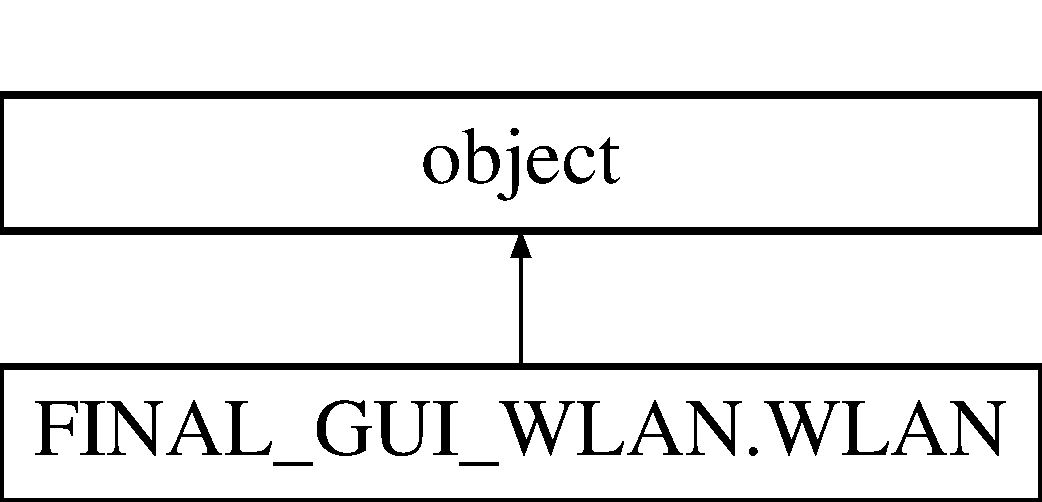
\includegraphics[height=2.000000cm]{class_f_i_n_a_l___g_u_i___w_l_a_n_1_1_w_l_a_n}
\end{center}
\end{figure}
\subsection*{Public Member Functions}
\begin{DoxyCompactItemize}
\item 
\mbox{\Hypertarget{class_f_i_n_a_l___g_u_i___w_l_a_n_1_1_w_l_a_n_abd0bb3e25ffdc1d77064fdbe4fae547c}\label{class_f_i_n_a_l___g_u_i___w_l_a_n_1_1_w_l_a_n_abd0bb3e25ffdc1d77064fdbe4fae547c}} 
def {\bfseries \+\_\+\+\_\+init\+\_\+\+\_\+} (self)
\item 
\mbox{\Hypertarget{class_f_i_n_a_l___g_u_i___w_l_a_n_1_1_w_l_a_n_a2253446c57d221d8374f492d3b039edf}\label{class_f_i_n_a_l___g_u_i___w_l_a_n_1_1_w_l_a_n_a2253446c57d221d8374f492d3b039edf}} 
def {\bfseries setup\+\_\+window} (self)
\item 
\mbox{\Hypertarget{class_f_i_n_a_l___g_u_i___w_l_a_n_1_1_w_l_a_n_ae429bf3b670d0b265edc4b1a220d9c6a}\label{class_f_i_n_a_l___g_u_i___w_l_a_n_1_1_w_l_a_n_ae429bf3b670d0b265edc4b1a220d9c6a}} 
def {\bfseries on\+\_\+close} (self)
\item 
def \hyperlink{class_f_i_n_a_l___g_u_i___w_l_a_n_1_1_w_l_a_n_a5fe71f63b3060bb7a5d1511aa0eeaf1c}{setup\+\_\+content} (self)
\item 
\mbox{\Hypertarget{class_f_i_n_a_l___g_u_i___w_l_a_n_1_1_w_l_a_n_a8a83ac894d6cdbc7a12003dcd2a1d274}\label{class_f_i_n_a_l___g_u_i___w_l_a_n_1_1_w_l_a_n_a8a83ac894d6cdbc7a12003dcd2a1d274}} 
def {\bfseries on\+\_\+received} (self)
\item 
\mbox{\Hypertarget{class_f_i_n_a_l___g_u_i___w_l_a_n_1_1_w_l_a_n_a8dd7e606685fb67b54e2c53626e46fba}\label{class_f_i_n_a_l___g_u_i___w_l_a_n_1_1_w_l_a_n_a8dd7e606685fb67b54e2c53626e46fba}} 
def {\bfseries senden} (self)
\item 
\mbox{\Hypertarget{class_f_i_n_a_l___g_u_i___w_l_a_n_1_1_w_l_a_n_aa39317ec4b35d7765ffbbefa3a341935}\label{class_f_i_n_a_l___g_u_i___w_l_a_n_1_1_w_l_a_n_aa39317ec4b35d7765ffbbefa3a341935}} 
def {\bfseries case\+\_\+1} (self, event)
\item 
\mbox{\Hypertarget{class_f_i_n_a_l___g_u_i___w_l_a_n_1_1_w_l_a_n_ae350f0f04417a03ebbde210d60553283}\label{class_f_i_n_a_l___g_u_i___w_l_a_n_1_1_w_l_a_n_ae350f0f04417a03ebbde210d60553283}} 
def {\bfseries case\+\_\+2} (self, event)
\item 
\mbox{\Hypertarget{class_f_i_n_a_l___g_u_i___w_l_a_n_1_1_w_l_a_n_a7f8af09fe47e662758efbe42031b3fb8}\label{class_f_i_n_a_l___g_u_i___w_l_a_n_1_1_w_l_a_n_a7f8af09fe47e662758efbe42031b3fb8}} 
def {\bfseries case\+\_\+3} (self, event)
\item 
\mbox{\Hypertarget{class_f_i_n_a_l___g_u_i___w_l_a_n_1_1_w_l_a_n_a6a47080307455eebf0bca74834d01077}\label{class_f_i_n_a_l___g_u_i___w_l_a_n_1_1_w_l_a_n_a6a47080307455eebf0bca74834d01077}} 
def {\bfseries case\+\_\+4} (self, event)
\item 
\mbox{\Hypertarget{class_f_i_n_a_l___g_u_i___w_l_a_n_1_1_w_l_a_n_ab52a928c6ffe8d1e58187b82c485bc41}\label{class_f_i_n_a_l___g_u_i___w_l_a_n_1_1_w_l_a_n_ab52a928c6ffe8d1e58187b82c485bc41}} 
def {\bfseries case\+\_\+5} (self, event)
\item 
\mbox{\Hypertarget{class_f_i_n_a_l___g_u_i___w_l_a_n_1_1_w_l_a_n_a508d6895200febe57522b7cb719da925}\label{class_f_i_n_a_l___g_u_i___w_l_a_n_1_1_w_l_a_n_a508d6895200febe57522b7cb719da925}} 
def {\bfseries case\+\_\+6} (self, event)
\item 
\mbox{\Hypertarget{class_f_i_n_a_l___g_u_i___w_l_a_n_1_1_w_l_a_n_a49ef4e8a9cf99463eef06e7607511c2f}\label{class_f_i_n_a_l___g_u_i___w_l_a_n_1_1_w_l_a_n_a49ef4e8a9cf99463eef06e7607511c2f}} 
def {\bfseries case\+\_\+7} (self, event)
\item 
\mbox{\Hypertarget{class_f_i_n_a_l___g_u_i___w_l_a_n_1_1_w_l_a_n_a3eddec1de07193250a7593ae4dd4b143}\label{class_f_i_n_a_l___g_u_i___w_l_a_n_1_1_w_l_a_n_a3eddec1de07193250a7593ae4dd4b143}} 
def {\bfseries case\+\_\+8} (self, event)
\item 
\mbox{\Hypertarget{class_f_i_n_a_l___g_u_i___w_l_a_n_1_1_w_l_a_n_ad19edd013fc170682baac727057a5155}\label{class_f_i_n_a_l___g_u_i___w_l_a_n_1_1_w_l_a_n_ad19edd013fc170682baac727057a5155}} 
def {\bfseries case\+\_\+9} (self, event)
\item 
\mbox{\Hypertarget{class_f_i_n_a_l___g_u_i___w_l_a_n_1_1_w_l_a_n_ad9a73c955c581f35964a55f79b9891ec}\label{class_f_i_n_a_l___g_u_i___w_l_a_n_1_1_w_l_a_n_ad9a73c955c581f35964a55f79b9891ec}} 
def {\bfseries case\+\_\+10} (self, event)
\item 
\mbox{\Hypertarget{class_f_i_n_a_l___g_u_i___w_l_a_n_1_1_w_l_a_n_a0727b5c8ed1339b9c3a5bc7c290a9502}\label{class_f_i_n_a_l___g_u_i___w_l_a_n_1_1_w_l_a_n_a0727b5c8ed1339b9c3a5bc7c290a9502}} 
def {\bfseries case\+\_\+standard} (self, event)
\item 
\mbox{\Hypertarget{class_f_i_n_a_l___g_u_i___w_l_a_n_1_1_w_l_a_n_aaeaf91e8d510f91d1830a4b428354de8}\label{class_f_i_n_a_l___g_u_i___w_l_a_n_1_1_w_l_a_n_aaeaf91e8d510f91d1830a4b428354de8}} 
def {\bfseries case\+\_\+schneller} (self, event)
\item 
\mbox{\Hypertarget{class_f_i_n_a_l___g_u_i___w_l_a_n_1_1_w_l_a_n_a00166245d4f6c4df9e40ecaffa66d0eb}\label{class_f_i_n_a_l___g_u_i___w_l_a_n_1_1_w_l_a_n_a00166245d4f6c4df9e40ecaffa66d0eb}} 
def {\bfseries case\+\_\+schnell} (self, event)
\item 
\mbox{\Hypertarget{class_f_i_n_a_l___g_u_i___w_l_a_n_1_1_w_l_a_n_afa11b6a032018490f3f7e7c9d2efd0bf}\label{class_f_i_n_a_l___g_u_i___w_l_a_n_1_1_w_l_a_n_afa11b6a032018490f3f7e7c9d2efd0bf}} 
def {\bfseries case\+\_\+mittelaf} (self, event)
\item 
\mbox{\Hypertarget{class_f_i_n_a_l___g_u_i___w_l_a_n_1_1_w_l_a_n_a5b05b7870d7878a5acc142d81c908b2b}\label{class_f_i_n_a_l___g_u_i___w_l_a_n_1_1_w_l_a_n_a5b05b7870d7878a5acc142d81c908b2b}} 
def {\bfseries case\+\_\+mittel} (self, event)
\item 
\mbox{\Hypertarget{class_f_i_n_a_l___g_u_i___w_l_a_n_1_1_w_l_a_n_a307f1abe3cdb76fb877c4267dceb0c82}\label{class_f_i_n_a_l___g_u_i___w_l_a_n_1_1_w_l_a_n_a307f1abe3cdb76fb877c4267dceb0c82}} 
def {\bfseries case\+\_\+langsamer} (self, event)
\item 
\mbox{\Hypertarget{class_f_i_n_a_l___g_u_i___w_l_a_n_1_1_w_l_a_n_acc83d940a64c2af519b20fb3b0f1875d}\label{class_f_i_n_a_l___g_u_i___w_l_a_n_1_1_w_l_a_n_acc83d940a64c2af519b20fb3b0f1875d}} 
def {\bfseries case\+\_\+langsam} (self, event)
\item 
\mbox{\Hypertarget{class_f_i_n_a_l___g_u_i___w_l_a_n_1_1_w_l_a_n_a0a597b89e22f363d7fe7e01e561693b4}\label{class_f_i_n_a_l___g_u_i___w_l_a_n_1_1_w_l_a_n_a0a597b89e22f363d7fe7e01e561693b4}} 
def {\bfseries run} (self)
\end{DoxyCompactItemize}
\subsection*{Public Attributes}
\begin{DoxyCompactItemize}
\item 
\mbox{\Hypertarget{class_f_i_n_a_l___g_u_i___w_l_a_n_1_1_w_l_a_n_a5d17d6eac4548c131d36e9ef29d6482a}\label{class_f_i_n_a_l___g_u_i___w_l_a_n_1_1_w_l_a_n_a5d17d6eac4548c131d36e9ef29d6482a}} 
{\bfseries arduino}
\item 
\mbox{\Hypertarget{class_f_i_n_a_l___g_u_i___w_l_a_n_1_1_w_l_a_n_a14f8296fbc442af46e469c22a237af0f}\label{class_f_i_n_a_l___g_u_i___w_l_a_n_1_1_w_l_a_n_a14f8296fbc442af46e469c22a237af0f}} 
{\bfseries h}
\item 
\mbox{\Hypertarget{class_f_i_n_a_l___g_u_i___w_l_a_n_1_1_w_l_a_n_a8cbd728602e35c20cf8de51cd306daf9}\label{class_f_i_n_a_l___g_u_i___w_l_a_n_1_1_w_l_a_n_a8cbd728602e35c20cf8de51cd306daf9}} 
{\bfseries i}
\item 
\mbox{\Hypertarget{class_f_i_n_a_l___g_u_i___w_l_a_n_1_1_w_l_a_n_adbb647739c0e9a6df01a051f9257ec92}\label{class_f_i_n_a_l___g_u_i___w_l_a_n_1_1_w_l_a_n_adbb647739c0e9a6df01a051f9257ec92}} 
{\bfseries j}
\item 
\mbox{\Hypertarget{class_f_i_n_a_l___g_u_i___w_l_a_n_1_1_w_l_a_n_a26b750ac9d82096cef0b35f20466386d}\label{class_f_i_n_a_l___g_u_i___w_l_a_n_1_1_w_l_a_n_a26b750ac9d82096cef0b35f20466386d}} 
{\bfseries k}
\item 
\mbox{\Hypertarget{class_f_i_n_a_l___g_u_i___w_l_a_n_1_1_w_l_a_n_a04274bdee217237704cf0b73b8ad7fb7}\label{class_f_i_n_a_l___g_u_i___w_l_a_n_1_1_w_l_a_n_a04274bdee217237704cf0b73b8ad7fb7}} 
{\bfseries l}
\item 
\mbox{\Hypertarget{class_f_i_n_a_l___g_u_i___w_l_a_n_1_1_w_l_a_n_ae6c3edea1b27b9e986b6ecc124effdec}\label{class_f_i_n_a_l___g_u_i___w_l_a_n_1_1_w_l_a_n_ae6c3edea1b27b9e986b6ecc124effdec}} 
{\bfseries m}
\item 
\mbox{\Hypertarget{class_f_i_n_a_l___g_u_i___w_l_a_n_1_1_w_l_a_n_a306c263936bc117701e855307e917e32}\label{class_f_i_n_a_l___g_u_i___w_l_a_n_1_1_w_l_a_n_a306c263936bc117701e855307e917e32}} 
{\bfseries n}
\item 
\mbox{\Hypertarget{class_f_i_n_a_l___g_u_i___w_l_a_n_1_1_w_l_a_n_a752538bc396704ac4602b652bf1c67db}\label{class_f_i_n_a_l___g_u_i___w_l_a_n_1_1_w_l_a_n_a752538bc396704ac4602b652bf1c67db}} 
{\bfseries o}
\item 
\mbox{\Hypertarget{class_f_i_n_a_l___g_u_i___w_l_a_n_1_1_w_l_a_n_a27dc01c12bb7da35a2353c185dfae508}\label{class_f_i_n_a_l___g_u_i___w_l_a_n_1_1_w_l_a_n_a27dc01c12bb7da35a2353c185dfae508}} 
{\bfseries a}
\item 
\mbox{\Hypertarget{class_f_i_n_a_l___g_u_i___w_l_a_n_1_1_w_l_a_n_a0763deac00958870b0220fbde25f5a44}\label{class_f_i_n_a_l___g_u_i___w_l_a_n_1_1_w_l_a_n_a0763deac00958870b0220fbde25f5a44}} 
{\bfseries b}
\item 
\mbox{\Hypertarget{class_f_i_n_a_l___g_u_i___w_l_a_n_1_1_w_l_a_n_af2eda9177ae53463c235655136bca0b7}\label{class_f_i_n_a_l___g_u_i___w_l_a_n_1_1_w_l_a_n_af2eda9177ae53463c235655136bca0b7}} 
{\bfseries c}
\item 
\mbox{\Hypertarget{class_f_i_n_a_l___g_u_i___w_l_a_n_1_1_w_l_a_n_a1ce5ec44ae3c588d8cb61a6197adfa58}\label{class_f_i_n_a_l___g_u_i___w_l_a_n_1_1_w_l_a_n_a1ce5ec44ae3c588d8cb61a6197adfa58}} 
{\bfseries d}
\item 
\mbox{\Hypertarget{class_f_i_n_a_l___g_u_i___w_l_a_n_1_1_w_l_a_n_a9e2f7fd26b1a9c2529835b6233b77a5b}\label{class_f_i_n_a_l___g_u_i___w_l_a_n_1_1_w_l_a_n_a9e2f7fd26b1a9c2529835b6233b77a5b}} 
{\bfseries e}
\item 
\mbox{\Hypertarget{class_f_i_n_a_l___g_u_i___w_l_a_n_1_1_w_l_a_n_a65a328c8eeb5db8fe43c5ac8f8eb26d8}\label{class_f_i_n_a_l___g_u_i___w_l_a_n_1_1_w_l_a_n_a65a328c8eeb5db8fe43c5ac8f8eb26d8}} 
{\bfseries f}
\end{DoxyCompactItemize}
\subsection*{Static Public Attributes}
\begin{DoxyCompactItemize}
\item 
\mbox{\Hypertarget{class_f_i_n_a_l___g_u_i___w_l_a_n_1_1_w_l_a_n_aeac6709da443ca41de175c549eb0caa7}\label{class_f_i_n_a_l___g_u_i___w_l_a_n_1_1_w_l_a_n_aeac6709da443ca41de175c549eb0caa7}} 
{\bfseries x}
\item 
\mbox{\Hypertarget{class_f_i_n_a_l___g_u_i___w_l_a_n_1_1_w_l_a_n_a720cbd5ab0bfa70f33b4df4d9eb5f1fb}\label{class_f_i_n_a_l___g_u_i___w_l_a_n_1_1_w_l_a_n_a720cbd5ab0bfa70f33b4df4d9eb5f1fb}} 
{\bfseries window}
\item 
\mbox{\Hypertarget{class_f_i_n_a_l___g_u_i___w_l_a_n_1_1_w_l_a_n_a0ae2586e259735d79d24bc6cf90028b6}\label{class_f_i_n_a_l___g_u_i___w_l_a_n_1_1_w_l_a_n_a0ae2586e259735d79d24bc6cf90028b6}} 
{\bfseries text}
\item 
\mbox{\Hypertarget{class_f_i_n_a_l___g_u_i___w_l_a_n_1_1_w_l_a_n_a6eeb65cc4d61327e371a6e387b1cdf2b}\label{class_f_i_n_a_l___g_u_i___w_l_a_n_1_1_w_l_a_n_a6eeb65cc4d61327e371a6e387b1cdf2b}} 
{\bfseries font}
\item 
\mbox{\Hypertarget{class_f_i_n_a_l___g_u_i___w_l_a_n_1_1_w_l_a_n_a28d6012cc35be2a2cd22a5b076c8120d}\label{class_f_i_n_a_l___g_u_i___w_l_a_n_1_1_w_l_a_n_a28d6012cc35be2a2cd22a5b076c8120d}} 
{\bfseries variable}
\item 
\mbox{\Hypertarget{class_f_i_n_a_l___g_u_i___w_l_a_n_1_1_w_l_a_n_acef6c9f6008d440075ab4c3abf3f1587}\label{class_f_i_n_a_l___g_u_i___w_l_a_n_1_1_w_l_a_n_acef6c9f6008d440075ab4c3abf3f1587}} 
{\bfseries p}
\item 
\mbox{\Hypertarget{class_f_i_n_a_l___g_u_i___w_l_a_n_1_1_w_l_a_n_a582d45150d973913b12e7254915d4ad9}\label{class_f_i_n_a_l___g_u_i___w_l_a_n_1_1_w_l_a_n_a582d45150d973913b12e7254915d4ad9}} 
{\bfseries value}
\item 
\mbox{\Hypertarget{class_f_i_n_a_l___g_u_i___w_l_a_n_1_1_w_l_a_n_aae67fe842d0706519efdfb4555a5fefd}\label{class_f_i_n_a_l___g_u_i___w_l_a_n_1_1_w_l_a_n_aae67fe842d0706519efdfb4555a5fefd}} 
{\bfseries command}
\item 
\mbox{\Hypertarget{class_f_i_n_a_l___g_u_i___w_l_a_n_1_1_w_l_a_n_a6104642e833ec3c75685f2632fc9de90}\label{class_f_i_n_a_l___g_u_i___w_l_a_n_1_1_w_l_a_n_a6104642e833ec3c75685f2632fc9de90}} 
{\bfseries y}
\item 
\mbox{\Hypertarget{class_f_i_n_a_l___g_u_i___w_l_a_n_1_1_w_l_a_n_aabd629581a558bbccec717f8ee9f6acf}\label{class_f_i_n_a_l___g_u_i___w_l_a_n_1_1_w_l_a_n_aabd629581a558bbccec717f8ee9f6acf}} 
{\bfseries q}
\item 
\mbox{\Hypertarget{class_f_i_n_a_l___g_u_i___w_l_a_n_1_1_w_l_a_n_a061fd8c9d4ae910e85b9812ae59a3f5d}\label{class_f_i_n_a_l___g_u_i___w_l_a_n_1_1_w_l_a_n_a061fd8c9d4ae910e85b9812ae59a3f5d}} 
{\bfseries r}
\item 
\mbox{\Hypertarget{class_f_i_n_a_l___g_u_i___w_l_a_n_1_1_w_l_a_n_a73feeffba511def562d112e6edfe2d27}\label{class_f_i_n_a_l___g_u_i___w_l_a_n_1_1_w_l_a_n_a73feeffba511def562d112e6edfe2d27}} 
{\bfseries s}
\item 
\mbox{\Hypertarget{class_f_i_n_a_l___g_u_i___w_l_a_n_1_1_w_l_a_n_ac28a8c7fd724ed38e5845c69c365363b}\label{class_f_i_n_a_l___g_u_i___w_l_a_n_1_1_w_l_a_n_ac28a8c7fd724ed38e5845c69c365363b}} 
{\bfseries t}
\item 
\mbox{\Hypertarget{class_f_i_n_a_l___g_u_i___w_l_a_n_1_1_w_l_a_n_ab2291c1d64851272bbe945178b0d05b2}\label{class_f_i_n_a_l___g_u_i___w_l_a_n_1_1_w_l_a_n_ab2291c1d64851272bbe945178b0d05b2}} 
{\bfseries u}
\item 
\mbox{\Hypertarget{class_f_i_n_a_l___g_u_i___w_l_a_n_1_1_w_l_a_n_a9c3477acb9bedac13149a4302e98b0c8}\label{class_f_i_n_a_l___g_u_i___w_l_a_n_1_1_w_l_a_n_a9c3477acb9bedac13149a4302e98b0c8}} 
{\bfseries skizze}
\item 
\mbox{\Hypertarget{class_f_i_n_a_l___g_u_i___w_l_a_n_1_1_w_l_a_n_a276f7d1e0be972de294dd7637470a407}\label{class_f_i_n_a_l___g_u_i___w_l_a_n_1_1_w_l_a_n_a276f7d1e0be972de294dd7637470a407}} 
{\bfseries file}
\item 
\mbox{\Hypertarget{class_f_i_n_a_l___g_u_i___w_l_a_n_1_1_w_l_a_n_a16a45d3298b67d332cda2260c9dbecce}\label{class_f_i_n_a_l___g_u_i___w_l_a_n_1_1_w_l_a_n_a16a45d3298b67d332cda2260c9dbecce}} 
{\bfseries skizze2}
\item 
\mbox{\Hypertarget{class_f_i_n_a_l___g_u_i___w_l_a_n_1_1_w_l_a_n_a03cca7b00a8470923485c6e196b063d6}\label{class_f_i_n_a_l___g_u_i___w_l_a_n_1_1_w_l_a_n_a03cca7b00a8470923485c6e196b063d6}} 
{\bfseries w}
\item 
\mbox{\Hypertarget{class_f_i_n_a_l___g_u_i___w_l_a_n_1_1_w_l_a_n_a17b149deff56b77cad88459300bbfaeb}\label{class_f_i_n_a_l___g_u_i___w_l_a_n_1_1_w_l_a_n_a17b149deff56b77cad88459300bbfaeb}} 
{\bfseries image}
\item 
\mbox{\Hypertarget{class_f_i_n_a_l___g_u_i___w_l_a_n_1_1_w_l_a_n_acfa0251fa33c37e6572e1e53403bee24}\label{class_f_i_n_a_l___g_u_i___w_l_a_n_1_1_w_l_a_n_acfa0251fa33c37e6572e1e53403bee24}} 
{\bfseries row}
\item 
\mbox{\Hypertarget{class_f_i_n_a_l___g_u_i___w_l_a_n_1_1_w_l_a_n_af2837a964bb00f10eea62088e5df550a}\label{class_f_i_n_a_l___g_u_i___w_l_a_n_1_1_w_l_a_n_af2837a964bb00f10eea62088e5df550a}} 
{\bfseries column}
\item 
\mbox{\Hypertarget{class_f_i_n_a_l___g_u_i___w_l_a_n_1_1_w_l_a_n_a8de62261cfda9f1ec5b09f9d99ef7492}\label{class_f_i_n_a_l___g_u_i___w_l_a_n_1_1_w_l_a_n_a8de62261cfda9f1ec5b09f9d99ef7492}} 
{\bfseries tempo}
\end{DoxyCompactItemize}


\subsection{Member Function Documentation}
\mbox{\Hypertarget{class_f_i_n_a_l___g_u_i___w_l_a_n_1_1_w_l_a_n_a5fe71f63b3060bb7a5d1511aa0eeaf1c}\label{class_f_i_n_a_l___g_u_i___w_l_a_n_1_1_w_l_a_n_a5fe71f63b3060bb7a5d1511aa0eeaf1c}} 
\index{F\+I\+N\+A\+L\+\_\+\+G\+U\+I\+\_\+\+W\+L\+A\+N\+::\+W\+L\+AN@{F\+I\+N\+A\+L\+\_\+\+G\+U\+I\+\_\+\+W\+L\+A\+N\+::\+W\+L\+AN}!setup\+\_\+content@{setup\+\_\+content}}
\index{setup\+\_\+content@{setup\+\_\+content}!F\+I\+N\+A\+L\+\_\+\+G\+U\+I\+\_\+\+W\+L\+A\+N\+::\+W\+L\+AN@{F\+I\+N\+A\+L\+\_\+\+G\+U\+I\+\_\+\+W\+L\+A\+N\+::\+W\+L\+AN}}
\subsubsection{\texorpdfstring{setup\+\_\+content()}{setup\_content()}}
{\footnotesize\ttfamily def F\+I\+N\+A\+L\+\_\+\+G\+U\+I\+\_\+\+W\+L\+A\+N.\+W\+L\+A\+N.\+setup\+\_\+content (\begin{DoxyParamCaption}\item[{}]{self }\end{DoxyParamCaption})}

\begin{DoxyVerb}Obere Buttons\end{DoxyVerb}
 

The documentation for this class was generated from the following file\+:\begin{DoxyCompactItemize}
\item 
F\+I\+N\+A\+L\+\_\+\+G\+U\+I\+\_\+\+W\+L\+A\+N.\+py\end{DoxyCompactItemize}

\chapter{Datei-\/\+Dokumentation}
\hypertarget{_f_i_n_a_l___g_u_i___w_l_a_n_8py}{}\section{Python/\+F\+I\+N\+A\+L\+\_\+\+G\+U\+I\+\_\+\+W\+L\+AN.py-\/\+Dateireferenz}
\label{_f_i_n_a_l___g_u_i___w_l_a_n_8py}\index{Python/\+F\+I\+N\+A\+L\+\_\+\+G\+U\+I\+\_\+\+W\+L\+A\+N.\+py@{Python/\+F\+I\+N\+A\+L\+\_\+\+G\+U\+I\+\_\+\+W\+L\+A\+N.\+py}}
\subsection*{Klassen}
\begin{DoxyCompactItemize}
\item 
class \hyperlink{class_f_i_n_a_l___g_u_i___w_l_a_n_1_1_arduino}{F\+I\+N\+A\+L\+\_\+\+G\+U\+I\+\_\+\+W\+L\+A\+N.\+Arduino}
\item 
class \hyperlink{class_f_i_n_a_l___g_u_i___w_l_a_n_1_1_w_l_a_n}{F\+I\+N\+A\+L\+\_\+\+G\+U\+I\+\_\+\+W\+L\+A\+N.\+W\+L\+AN}
\end{DoxyCompactItemize}
\subsection*{Namensbereiche}
\begin{DoxyCompactItemize}
\item 
 \hyperlink{namespace_f_i_n_a_l___g_u_i___w_l_a_n}{F\+I\+N\+A\+L\+\_\+\+G\+U\+I\+\_\+\+W\+L\+AN}
\end{DoxyCompactItemize}
\subsection*{Variablen}
\begin{DoxyCompactItemize}
\item 
\hyperlink{namespace_f_i_n_a_l___g_u_i___w_l_a_n_ace49c6e031d3bddfe51aef1314e55222}{F\+I\+N\+A\+L\+\_\+\+G\+U\+I\+\_\+\+W\+L\+A\+N.\+window} = W\+L\+AN()
\end{DoxyCompactItemize}

%--- End generated contents ---

% Index
\backmatter
\newpage
\phantomsection
\clearemptydoublepage
\addcontentsline{toc}{chapter}{Index}
\printindex

\end{document}
